\chapter{Word Embedding}
%Word embeddings is distributed representation of words in a vector space. With the learning algorithm it can capture the contextual or co-occurrence information. The word embedding has an interesting and important property: similar words will have similar distribution in the embedding space, with that property, we can find meaningful near-synonyms or  Some successful methods for learning word embedding like word2vec\cite{mikolov2013distributed}, \cite{pennington2014glove}
%Word embeddings, when used as the underlying input representation, have been shown to boost the performance in  neural network models for natural language processing (NLP) tasks such as sequence tagging and text classification.
Researchers have worked on a number of methods for using word embedding in MT tasks. It has been proven that word embedding helps to improve the translation quality and handle the Out-Of-Vocabulary (OOV) problems (\cite{neishi2017bag}, \cite{qi2018and}). Recently, cross-lingual word embedding is quickly gaining in popularity. They play a crucial role in transferring knowledge from one language to another. Cross-lingual word embeddings have been used either in standard machine translation system (\cite{lample2017unsupervised}) or as a method for learning translation lexicons in an entirely unsupervised manner (\cite{xing2015normalized}, \cite{lample2018phrase}). \\
%\cite{neishi2017bag} attempt initializing the embedding layers with pre-trained word embeddings on the training datasets in the source languages. They find such method can improve the translation quality.  \cite{qi2018and} point that pretrained embeddings seem to be more effective for more similar translation pairs and it helps most when the training data is not large enough. Word embedding are also exploited to handle the out-of-vocabulary (OOV) problem.\\
Before we discuss the cross-lingual word embedding in this chapter, I will first introduce the learning algorithm for monolingual word embedding.Then I will explain the training and the lexical translation inference methods.

\section{Monolingual Embedding}
%A large majority of cross-lingual embedding models take inspiration from and extend monolingual word embedding models to bilingual settings, or explicitly leverage monolingually trained models. As an important preliminary, we thus briefly introduce monolingual embedding models.
Word embedding is distributed representation of word in high dimensional space. It can capture the contextual or co-occurrence information, so that similar words have similar distribution in the embedding space.  Several methods have been proven to be success like word2vec (\cite{mikolov2013efficient}) GloVe (\cite{pennington2014glove})
\begin{figure}[h]
	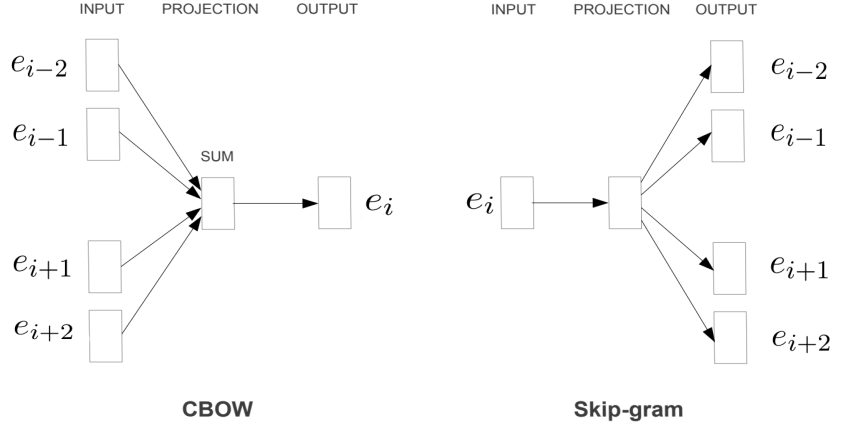
\includegraphics[width=12cm]{skip}
	\caption{Global attention model (\cite{mikolov2013efficient})}
	\centering
\end{figure}
\subsection{CBOW and Skip-gram}
CBOW and skip-gram are current mainstream neural network model to learn word embedding. Algorithmically,  CBOW tries to predict the current word based on the context while skip-gram model is to find better representations that are useful for predict \cite{qi2018and}ing the context words. Using skip-gram model as example, given a large training corpus represented as a sequence of words ${e_1^N: = e_1, \cdots e_I}$, the objective of the model is to maximize the following log-likelihood:
\[ \mathcal{L}^e_{\text{skip-gram}} = - \frac{1}{I} \sum_{i=1}^{I} \sum_{ -c \le d \le c, d\ne 0} \log\ {p(e_{i+d}|e_i)}\]

where $e_i$ is the current word and $c$ is the size of training context. \\


Similarly, we define the loss for CBOW model as
\[ \mathcal{L}^e_{\text{CBOW}} = - \frac{1}{I} \sum_{i=1}^{I} \sum_{ -c \le d \le c, d\ne 0} \log\ {p(e_{i}|e_{i+d})}\]


\subsection{GloVe}
Global vectors(GloVe) allows us to learn word representations via matrix factorization. GloVe minimizes the difference between the dot product of the embeddings of word and its context and the logarithm of their number of co-occurrences within a certain window size:
\[ \mathcal{L}_{GloVe}^e = \sum_{i,j=1}^{\lvert V_e \rvert} f(C_{ij})({\bm{e}_i}^{\top} \bm{e}_j - \log{C_{ij}} ) \]
where the matrix of word-word co-occurrence counts be denoted as $C$, whose entries $C_{ij}$ tabulate the number of times word $e_j$ occurs in the context of word $e_j$ and $f(\cdot)$ is a weighting function that assigns relatively lower weight to rare and frequent co-occurrences. $V_e$ is the source vocabulary size.
%Furthermore in skip-gram model, suppose given a scoring function s which maps word pairs to score in $\mathbb{R}0$ like cosine similarity, the probability can be defined as
%\[ p(e_{i+j} | e_i)  = \frac{\exp\{s(e_{i+j}, e_j)\}}{\sum_{e^{\prime} \in V^e }{\exp\{s( e^{\prime}, e_i)\}}}\]
%where $V^e$ is the whole vocabulary. \\
%
%\textbf{Negative Sampling}\\
%However the normalization on the whole vocabulary is very expensive since it is conducted for all words at every training step. Negative sampling is proposed to approximate the softmax to make it computationally more efficient. The problem of predicting words can be considered as an independent binary classification task. Negative sampling trains the model to distinguish a target word from negative samples drawn from a noise  distribution $P_{\text{noise}}$.   
%\[p(e_{i+j}|e_i) = \log {Q_{\theta}{(D=1 | e_{i+j}, e_i)}} + \frac{1}{k}\sum_{e^{\prime} \sim P_{\text{noise}}} {\log{Q_{\theta}{(D=0 | e^{\prime}, e_i )}}}  \]
%
%where ${Q_{\theta}{(D=1| w_t, w_s)}}$ is the binary logistic regression probability.
%According to  empirical results, CBOW works better on smaller datasets because CBOW smoothes over a lot of the distributional information while Skip-Gram model performs better when we have larger datasets
%
%\subsection{Enriching Embedding with Subword Information}
%The training methods above treat each word as a distinct word embedding, however intuitively we can obtain more information from the morphological information of words. A subword model was proposed to try to fix such problem.The training network is similar, the model design a new presentation of the word: it adds speicial symbols $<$, ${>}$ as boundary information at the beginning and the end of a word. Then a normal word is represented as a bag of character $n$-grams . For example the word "where" and n equals 3, the it can be represented as the following 5 tri-grams: 
%\[ <wh, whe, her, ere, re>\]
%Suppose in this way for a specific word $e$ ${G_{e}}$ the set of character ${n}$-grams, we assign for each character ${n}$-gram $g$ in ${G_{e}}$ a distinct vector $\bm{v}_g$, we calculate the score function using the sum of character-level inner product of vectors:
%\[s(e^{\prime}, e) = \sum_{g \in G_{e}} \bm{v}_g^{T} \bm{e}^{\prime} \]
%where $\bm{e}^{\prime}$ the embedding of $e^{\prime}$
\section{ Cross-lingual Word Embedding}
% NLP tasks in multilingual scenarios is receiving increasing interest. The need to represent meaning and transfer knowledge in cross-lingual applications has motivated the work on cross-lingual models, which learns the representations in a joint embedding space.
  \cite{mikolov2013exploiting}  observe that word embeddings trained separately on monolingual corpora exhibit isomorphic structure across languages, as illustrated in Figure $3.2$. That means we can create a connection between source embedding and target embedding even with simple linear mapping. This has far-reaching implication on low-resource scenarios (\cite{adams2017cross}), because word embedding training requires only plain text to train, which is the most abundant form of linguistic resource.
\begin{figure}[t]
	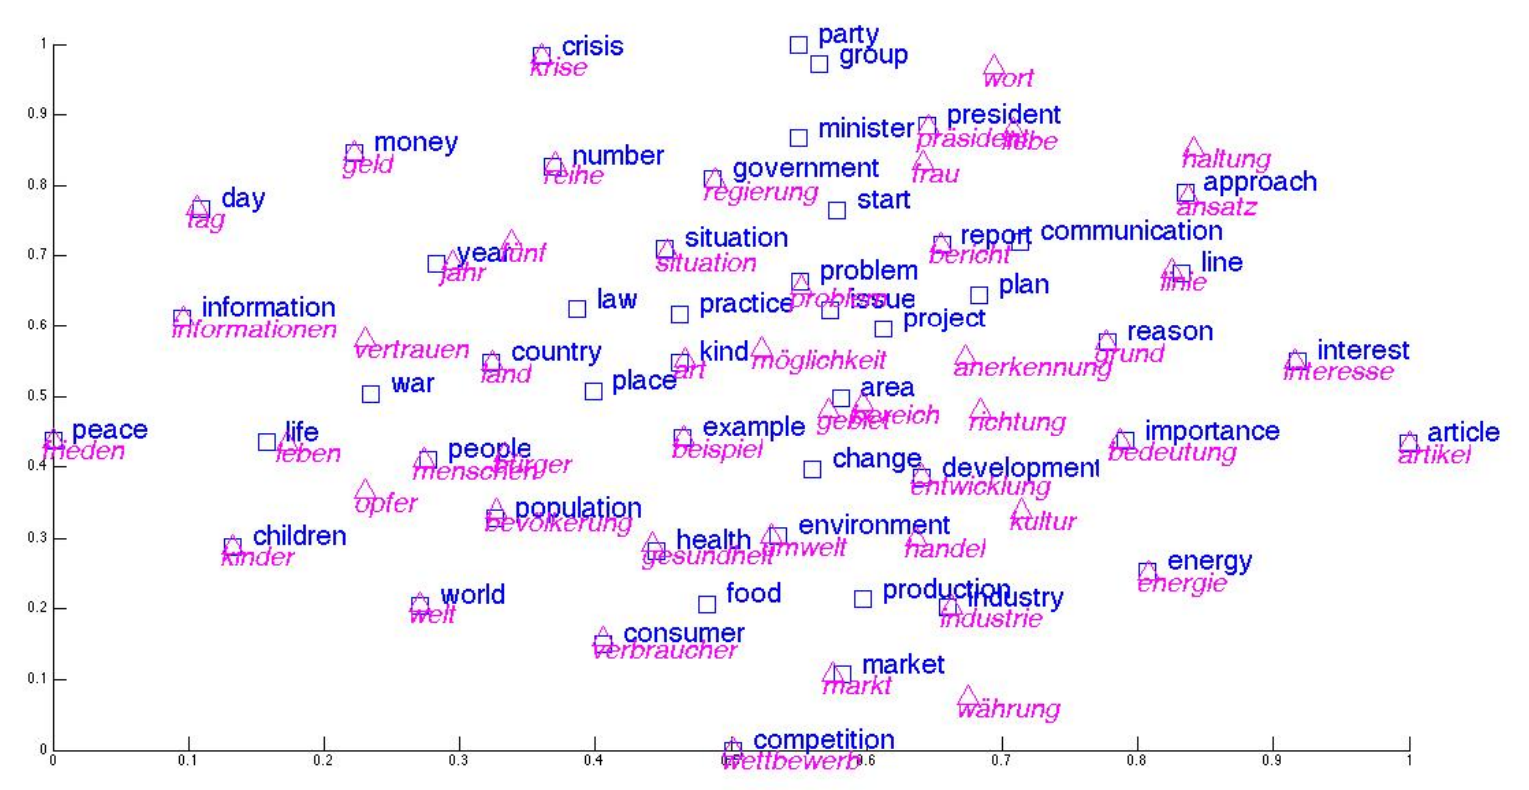
\includegraphics[width=14cm]{crossembedding}
	\centering
	\caption{A cross-lingual embedding space between German and English (\cite{ruder2017survey})}
\end{figure}

%In the thesis, I assume there are two set of embeddings ${e}$, ${f}$trained separately on monolingual data.  The propose of cross-lingual word embedding training is to learn such a mapping ${W \in }$ from source embedding space to target embedding space, so $Wf_i, e_j$ in the same embedding space and for all corresponding word pairs, we need to optimize the mapping ${W}$, so that"
%
%
%\[ \arg\min_{W \in R^{d \times d}} \sum_{i} \lVert Wf_i - e_i \rVert \]
%where $d$ is the dimension of embeddings, and the distance ${\lVert Wf_i - e_i \rVert}$ can be different types. We prefer the Euclidean distance.  
%
%first
	

\subsection{Supervised Training}
Before we go on to the main training setting of this thesis (unsupervised), I will introduce the training methods under supervision. The supervision comes from seed lexicons, parallel data or document-aligned data.\\
Supervised training methods of cross-lingual word embedding can be divided into joint training approaches and mapping-based approaches. The difference is that joint methods train directly the cross-lingual word embeddings, while the mapping-based approaches first train monolingual word representations on corresponding corpus separately. Then mapping will be learned to project different embeddings into a shared space according to supervision signals. \\

\textbf{Joint Training Approaches}\\
Here the joint training means to optimize source and target embedding objectives $\mathcal{L(\cdot)}$ together with the cross-lingual regularization term $\Omega(\cdot)$. 
\[ \mathcal{L} =  \mathcal{L}_{\text{mono}}^e + \mathcal{L}_{\text{mono}}^f + \cdot \Omega(\cdot)  \]
where the first two losses are exact the same as those in monolingual embedding training.  $\Omega(\cdot)$  encourages representations to be similar for words that are related across different languages.

Different cross-lingual regularization terms are proposed to optimize the cross-lingual embeddings (\cite{coulmance2016trans}, \cite{luong2015bilingual}, \cite{gouws2015bilbowa}). For example, \cite{gouws2015bilbowa} models it as: 
\[ \Omega_{\text{BilBOWA}} = \sum_{( f_1^J, e_1^I)}{\lVert \frac{1}{I}  \sum_{e_i \in e_1^I} \bm{e}_i - \frac{1}{J} \sum_{f_j \in f_1^J} \bm{f}_j\rVert}^2 \]
where $\bm{f}_j$ and $\bm{e}_i$ are the word embeddings for words in parallel source and target sentences $(f_1^J, e_1^I)$. Instead of relying on expensive word alignments which minimize the distance that aligned to each other, they minimize the distance between the mean of the word representations in the aligned sentences. \\

\textbf{Mapping-based Approaches}\\
Another approach is to train monolingual word representations separately on monolingual corpora and then learn a transformation matrix mapping that maps representations in one language to the representations of other language.  This approach can be further divided into learning separate mappings for each language or learning mapping only for source language to project source embeddings into target embedding space.

learn the transformation for each language, both monolingual embeddings are mapped into a shared embedding space. The typical model is CCA-based approaches (\cite{faruqui2014improving}, \cite{dhillon2011multi} and \cite{lu2015deep}). The other method is to learn the mapping from the source embedding space to the target embedding space. The criterion is to minimize the mean squared error between the transformed source embeddings and the target embeddings. The advantage of this method is that it is really fast to learn the embeddings and embedding alignments. People criticize whether linear or nonlinear can capture the relationship between all words in different languages.
\begin{itemize}
	\item Mapping matrix for each language\\
	The typical method is  canonical correlation analysis(CCA).
	\begin{figure}[t]
		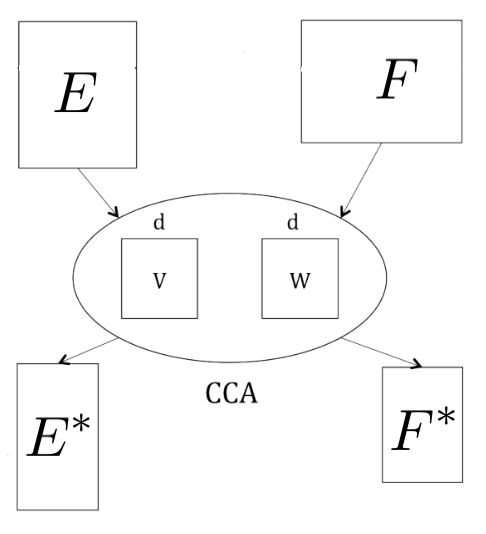
\includegraphics[width=8cm]{cca}
		\centering
		\caption{Cross-lingual projection with CCA (\cite{faruqui2014improving})}
	\end{figure}
	let $F $ and $E$ be the embedding matrices comprised of seed word translation pairs. The  $W$ and $V$ are the projection matrices which mapped the original embedding matrices into $F^{*}$ and $E^{*}$, which are in the joint space, $d$ is the embedding dimension.
	
	\[ {F}^{*} = W{F} \ \ \ \  {E}^{*} = V{E} \] 
	The objective of CCA is to find the two matrices such that the projections of the parallel matrices are maximally correlated:
	\begin{align}
		W^*, V^* =& \argmax{W, V \in \mathbb{R}^{d \times d}} \text{corr}(WF, VE)\\
		= &\argmax{W, V \in \mathbb{R}^{d \times d}} \frac{\mathbb{E}[(W{F})(V{E})]}{\sqrt{\mathbb{E}[(W{F})^2]} \sqrt{\mathbb{E}[( V{E})^2]}}
	\end{align}

	Once we get the two projection matrices, we can calculate the cross-lingual word embedding for the entire source and target vocabulary.
	
	A linear feature mapping is often not sufficiently powerful to faithfully capture the hidden, non-linear relations within the data. \cite{lu2015deep} propose a non-linear extension of CCA using deep neural networks to maximize the
	correlation between the projections of both monolingual embedding spaces
	\[ f_1^*, f_2^* = \argmax{f_1, f_2} \ \text{corr}(f_1(F), f_2(E)) \]
	where $f_1$ and $f_2$ are non-linear transformation implemented by neural networks.
	
	\item Mapping matrix for only source language
	\cite{mikolov2013exploiting} notice that the geometric relation that hold between words are similar across languages. This suggest that, we can learn the transformation directly from source embedding space to target space.
	Given a seed word translation pair set $dico$, the objective is to learn $W$ that minimizes the distance between mapped source word embedding $W\bm{f}$ and corresponding target embedding $\bm{e}$:
	\[ \argmin{W} \sum_{(\bm{f}, \bm{e}) \in dico}  {\lVert W\bm{f} - \bm{e} \rVert}_2^2 \]
	This can also be expressed in matrix form as minimizing the squared Frobenius norm of the residual matrix $F$, $E$:
	\[ \argmin{W} {\ \lVert WF - E \rVert}_{\text{F}}^2 \]
	
	
	
	\cite{xing2015normalized} showed that the results are improved when we use $l_2$ normalized embeddings and constrain the ${W}$ to be an orthogonal matrix. In this case we can use Procrustes analysis which advantageously offers a closed form solution obtained from the singular value decomposition 
	\[W^* = \argmin{W \in O_d(\mathbb{R})} {\ \lVert WF - E \rVert}_{\text{F}}^2 = UV^T , \quad U\Sigma V^T = \text{SVD}(EF^T) \]
	where $ O_d(\mathbb{R})$ denotes manifold of orthogonal matrices 
\end{itemize}


\[ \]
%where $W_f$ and $W_e$ are the weights of the two networks and ${}$ ${}$, ${}$ are covariance matrices computed for   in the ssame way as CCA. The final transformation is the composition of the neural network ans CCA projection, $\bm{u}^T \bm{f}$ for the view. The algorithm does not have a closed-form solution but the parameters can be learned via gradient-based optimization with mini-batch stochastic gradient descent .
%\begin{enumerate}
%	\item Mapping based approaches\\
%	First train the monolingual word embedding separately and then seek the seed dictionary to learn the mapping. 
%	\item Pseudo-multi-lingual corpora-based approaches\\
%	Use the monolingual embedding training method on constructed corpora that contains both the source and the target language.
%	\item Joint methods\\
%	Take the parallel text as input and minimize the source and target language losses jointly with the cross-lingual regularization term
%\end{enumerate}





%In order to make learning and inference consistent, \cite{DBLP:journals/corr/abs-1804-07745} propose the relaxed CSLS loss (RCSLS), which is inspired from the work of \cite{conneau2017word}
%
%The loss function can be rewritten as:
%\[ \min_{\bm{W} \in \mathcal{O}_d} = \frac{1}{n} \sum_{i=1}^{n} \Big\{ -2 \bm{f}_i^\top W^\top \bm{e}_i + \frac{1}{k} \sum_{\bm{e}_j \in \mathcal{N}_e(W\bm{f}_i)} \bm{f}_i^\top W^\top \bm{e}^j + \frac{1}{k} \sum_{W\bm{f}_j \in \mathcal{N}_f(\bm{e}_i)} \bm{f}_j^\top W^\top \bm{e}^i  \Big\}\]

%
%Normally, the size $n$ of the dictionary is too small with respect to the entire vocabulary size, in order to incorporate unlabeled data, the unpaired words in the dictionary are used as "negatives samples" in the RCSLS loss, as result, we can optimize the loss function not only the dictionary but the whole vocabulary.

\subsection{Biligual Lexicon Induction}
When we use nearest neighbors search to infer the word translation, we suffer from the so-called "hubness Problem": points are tending to be nearest neighbors of many points in high-dimensional space.  Those points (hubs) will harm the search accuracy.\\
Now this limitation is addressed by apply a applying a corrective metric at inference time, such as inverted softmax (ISF)(\cite{smith2017offline})  or cross-domain similarity scaling (CSLS)(\cite{conneau2017word})
\begin{itemize}
	\item Inverted Softmax (ISF)\\
	The confidence of choosing a target word as translation of a source word can be considered as softmax-like normalized probability
	\[ p(e|f) = \frac{\exp{\Big(\beta \cdot  \text{score}(e,f)\Big)}}{\sum_{e^{\prime}} {\exp{\Big(\beta \cdot \text{score}(e^{\prime}, f)\Big)}}} \]
	where the $\text{score}(\cdot)$ is the score function we can define ourselves.
	we learn the "temperature" $\beta$ by maximizing the log probability over the training dictionary. 
	\[ \argmax{\beta} \sum_{e,f} \ln p(e|f)  \]
	
	The author observed that, if we invert the softmax and normalizing the probability over all the source words rather than target words, the hubness problem could be mitigated:
	\[ p(e|f) = \frac{\exp{\Big(\beta \cdot  \text{score}(e,f)\Big)}}{\alpha \  \sum_{f^{\prime}} {\exp{\Big(\beta \cdot \text{score}(e, f^{\prime})\Big)}}}\]
	\item  Cross-domain Similarity Local Scaling (CSLS)\\
	We denote ${\mathcal{N}_e(\bm{f})}$ the set of ${k}$ nearest neighbors of points of the mapped $\bm{f}$ in the target embedding space, and ${\mathcal{N}_f(\bm{e})}$ the nearest neighbors of mapped ${\bm{e}}$ in the source embedding space. We consider the mean cosine similarity as hub-ness:
	\[ r(\bm{f})= \frac{1}{K} \sum_{\bm{e}^{\prime} \in \mathcal{N}_e(\bm{f})} \cos(\bm{e}^{\prime}, W\bm{f})\]
	So in this way we penalize the hub points:
	\[ CSLS(\bm{e}, \bm{f}) = 2 \cos(\bm{e}, \bm{f}) - \frac{1}{k} \sum_{\bm{e^{\prime}} \in \mathcal{N}_e(\bm{f})} \cos(\bm{f}, \bm{e^{\prime}})- \frac{1}{k} \sum_{\bm{f^{\prime}} \in \mathcal{N}_f(\bm{e})} cos(\bm{f^{\prime}}, \bm{e}) \]
\end{itemize}


%Since we use the pseudo parallel data (source sentence and word-by-word target translation sentence), we can exploit the context information from language model to select the word translation candidate. Beam search with language model is implemented here. More details about sentence translation will be explained next chapter.\\
